\documentclass[journal,10pt,onecolumn,draftclsnofoot]{IEEEtran}
\usepackage{cite}
\usepackage{amsmath,amssymb,amsfonts}
\usepackage{algorithmic}
\usepackage{graphicx}
\usepackage{textcomp}
\usepackage{xcolor}
\usepackage{booktabs}
\usepackage{array}
\usepackage{url}
\usepackage{tikz}
\usetikzlibrary{shapes,arrows,positioning,calc}

\begin{document}

\title{Explainable Multimodal Deepfake Detection System via Attention-Weighted Cross-Modal Evidence Aggregation and Temporal Boundary Localization}

\author{Vineeth Prabhu,~\IEEEmembership{Student Member,~IEEE,}
        and Research Collaborators
\thanks{V. Prabhu is with the Department of Artificial Intelligence and Data Science, NMAM Institute of Technology, NITTE (Deemed to be University), Mangaluru, India (e-mail: nnm24ad071@nmamit.in).}}

\markboth{IEEE Transactions on Information Forensics and Security,~Vol.~XX, No.~X, July~2026}%
{Prabhu \MakeLowercase{\textit{et al.}}: Explainable Multimodal Deepfake Detection System}

\maketitle

\begin{abstract}
The alarming proliferation of sophisticated generative models, face reenactment tools, and speech synthesis algorithms has undermined the authenticity of digital media. Modern deepfakes are increasingly multimodal, combining visual manipulations with synthetic voice cloning or manipulated lip synchronization. Consequently, single-modality detectors that evaluate only visual artifacts or acoustic patterns are insufficient, particularly against high-fidelity, dual-channel forgeries. This paper proposes a comprehensive, explainable Multimodal Deepfake Detection System (MDDS) that aggregates speech audio, face crops, and mouth regions using a cross-modal transformer fusion architecture. Our system utilizes a pretrained Wav2Vec2 backbone for robust speech representation, paired with dual Vision Transformer (ViT) encoders to capture identity and fine-grained visual articulation patterns. A cross-modal attention module dynamically aligns the audio and visual channels, passing representations to specialized forensic heads that score lip-sync mismatch, visual identity tampering, temporal discontinuity, and audio-visual synchronization anomalies. These channel outputs are aggregated using an attention-weighted Forensic Evidence Aggregator to generate a calibrated overall probability and confidence score. Furthermore, we integrate a Temporal Forgery Boundary Detector (TFBD) consisting of a 1D dilated CNN and a linear-chain Conditional Random Field (CRF) to precisely localize the start and end of tampered segments. We evaluate the proposed system on FakeAVCeleb, FaceForensics++, and LAV-DF. The system employs dataset-aware routing and threshold calibration to manage domain shift and precision-recall trade-offs. Ablation studies demonstrate that multimodal fusion significantly outperforms single-modality analysis, yielding a validation ROC-AUC of 0.9130 on FakeAVCeleb. In addition, we present a classical machine learning baseline using engineered feature fusion, where a Fusion XGBoost model achieves an F1-score of 0.8806 on FakeAVCeleb. The proposed MDDS framework outputs detailed JSON/HTML reports, frame-by-frame anomaly timelines, and spatial heatmap overlays, providing the level of explainability necessary for digital forensic investigations.
\end{abstract}

\begin{IEEEkeywords}
Deepfake detection, multimodal fusion, audio-visual forensics, cross-modal attention, temporal boundary localization, conditional random fields, explainable artificial intelligence.
\end{IEEEkeywords}

\section{Introduction}
\IEEEPARstart{T}{he} rapid evolution of deep generative models, particularly Generative Adversarial Networks (GANs) and diffusion architectures, has simplified the creation of highly realistic synthetic media. While these technologies have spurred positive applications in the entertainment, creative, and educational sectors, they pose substantial risks when exploited for malicious purposes. The fabrication of high-fidelity ``deepfakes''—synthetic videos depicting individuals saying or doing things they never did—has been used to spread misinformation, conduct financial fraud, commit political manipulation, and defame individuals. As these synthetic generation techniques continue to mature, the boundary between genuine and manipulated digital evidence has become increasingly blurred.

Early deepfake detection methodologies focused primarily on detecting visual artifacts within individual video frames. These methods analyzed abnormalities such as irregular blinking patterns, inconsistencies in ear and nose geometry, blending boundary artifacts, and color distribution anomalies. However, generative tools have quickly adapted, incorporating advanced face alignment, lighting normalization, and boundary-blending techniques that eliminate many of the low-level visual indicators targeted by early detectors. Furthermore, modern deepfakes are no longer restricted to visual face-swaps. They frequently incorporate synthetic voice cloning, text-to-speech rendering, and automated lip synchronization (e.g., Wav2Lip), resulting in highly coordinated multimodal manipulations. Consequently, visual-only forensic models can easily be bypassed if the visual rendering is flawless but the audio channel or the alignment between speech and lip movement is manipulated.

\begin{figure*}[htbp]
\centering
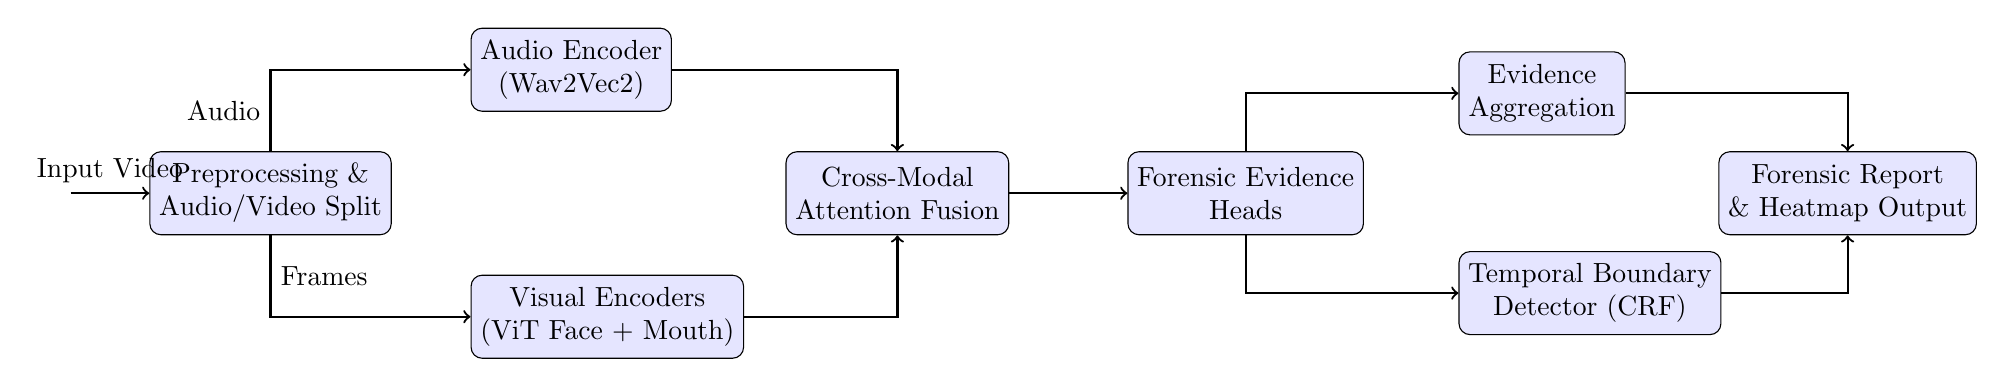
\begin{tikzpicture}[node distance=1.5cm, auto]
    \tikzstyle{block} = [draw, fill=blue!10, rectangle, minimum height=3em, minimum width=6em, rounded corners, align=center]
    \tikzstyle{input} = [coordinate]
    \tikzstyle{output} = [coordinate]
    \tikzstyle{pinstyle} = [pin edge={to-,t,black}]
    
    % Nodes
    \node [input] (input_video) {};
    \node [block, right=1cm of input_video] (preprocess) {Preprocessing \& \\ Audio/Video Split};
    \node [block, above right=0.5cm and 1cm of preprocess] (audio_enc) {Audio Encoder \\ (Wav2Vec2)};
    \node [block, below right=0.5cm and 1cm of preprocess] (video_enc) {Visual Encoders \\ (ViT Face + Mouth)};
    \node [block, right=5cm of preprocess] (fusion) {Cross-Modal \\ Attention Fusion};
    \node [block, right=1.5cm of fusion] (forensic_heads) {Forensic Evidence \\ Heads};
    \node [block, above right=0.2cm and 1.2cm of forensic_heads] (aggregator) {Evidence \\ Aggregation};
    \node [block, below right=0.2cm and 1.2cm of forensic_heads] (tfbd) {Temporal Boundary \\ Detector (CRF)};
    \node [block, right=4.5cm of forensic_heads] (report) {Forensic Report \\ \& Heatmap Output};

    % Paths
    \draw [->, thick] (input_video) -- node {Input Video} (preprocess);
    \draw [->, thick] (preprocess) |- node [near start] {Audio} (audio_enc);
    \draw [->, thick] (preprocess) |- node [near start] {Frames} (video_enc);
    \draw [->, thick] (audio_enc) -| (fusion);
    \draw [->, thick] (video_enc) -| (fusion);
    \draw [->, thick] (fusion) -- (forensic_heads);
    \draw [->, thick] (forensic_heads) |- (aggregator);
    \draw [->, thick] (forensic_heads) |- (tfbd);
    \draw [->, thick] (aggregator) -| (report);
    \draw [->, thick] (tfbd) -| (report);
\end{tikzpicture}
\caption{System architecture of the proposed Multimodal Deepfake Detection System (MDDS), showcasing raw preprocessing, dual encoder pipelines, cross-modal attention, specialized forensic heads, evidence aggregation, and temporal boundary localization.}
\label{fig:mdds_full_flow}
\end{figure*}

To counter multimodal deepfakes, the forensic research community has turned to audio-visual consistency analysis. A genuine video exhibits tight alignment between the acoustic properties of the speech, the phonemes spoken, the physical movement of the mouth, the emotional expressions of the speaker, and the global video continuity. When a video is synthesized, these channels frequently exhibit minor discrepancies due to limits in rendering accuracy, cross-modal timing offsets, or mismatch in speaker characteristics. Analyzing these cross-modal inconsistencies provides a promising and generalizable framework for deepfake detection, as it targets fundamental physical and behavioral relationships that are highly challenging for generators to synchronize perfectly.

However, existing multimodal deepfake detection models exhibit significant limitations that prevent their deployment in real-world forensic workflows:
\begin{enumerate}
    \item \textbf{Explainability Deficit:} Most models operate as black-box binary classifiers, outputting only a final ``real'' or ``fake'' label. They do not disclose which evidence channel (e.g., lip-sync anomaly, acoustic voice cloning, or visual boundary artifact) drove the decision, making them unsuitable for legal or expert forensic review.
    \item \textbf{Lack of Temporal Localization:} Standard detectors analyze whole videos and output a single score. They do not identify precisely \textit{when} a manipulation begins or ends within a clip. This is highly problematic because localized deepfakes might only be manipulated for a short fraction of the duration, allowing the remainder of the clip to dilute the anomaly score.
    \item \textbf{Calibration Mismatch:} Models trained on academic benchmarks exhibit severe score calibration shifts when deployed. Using a static threshold of $0.50$ across different codecs, compressions, or datasets leads to massive rates of false positives or false negatives.
\end{enumerate}

To address these limitations, this paper presents an explainable Multimodal Deepfake Detection System (MDDS) built around cross-modal attention, specialized forensic heads, attention-weighted evidence aggregation, and temporal CRF boundary decoding. Our system takes a raw video and decomposes it into audio and visual components. The audio channel is processed using a pretrained Wav2Vec2 network to extract high-dimensional speech features. The visual channel is split into two separate paths: a global Vision Transformer (ViT) to extract face identity and boundary cues, and a localized ViT to capture fine-grained lip and mouth articulation features. These streams are combined using a cross-modal transformer fusion layer that models the cross-attention between audio phoneme tokens and visual mouth movement frames. 

The fused features are passed to four independent forensic evidence heads, each trained to detect a specific anomaly: lip-synchronization error, visual identity mismatch, temporal discontinuity, and audio-video synchronization offset. The outputs of these heads are aggregated using an attention-weighted evidence aggregation layer that dynamically assigns weights to each channel based on their relevance to the sample. This produces a calibrated unified probability and confidence score. Simultaneously, the system extracts frame-by-frame anomalies and feeds them into a Temporal Forgery Boundary Detector (TFBD). The TFBD utilizes a 1D dilated CNN to model temporal context and a linear-chain Conditional Random Field (CRF) to decode the optimal sequence of frame labels (REAL, FAKE, or BOUNDARY), generating precise timestamps for the manipulated regions.

The remainder of this paper is structured as follows: Section II reviews related literature and highlights the research gap. Section III details the mathematical formulation and architecture of the proposed MDDS framework. Section IV describes the experimental setup, datasets, and hyperparameters. Section V evaluates the system's performance and presents calibration and classical ML baselines. Section VI discusses the modality ablation studies and explainability artifacts. Section VII discusses threats to validity and future directions. Section VIII concludes the paper.

\section{Related Work}
\subsection{Visual-Only Deepfake Detection}
Visual-only forensic techniques have formed the historical foundation of deepfake detection. Early models relied on detecting low-level blending artifacts, such as differences in color temperature, resolution mismatch between the cropped face and the background, or artifacts left by affine warping. Researchers have also proposed detecting high-level physiological indicators, such as lack of natural eye blinking, inconsistencies in ear and dental structure, and abnormal pulse signals derived from remote photoplethysmography (rPPG). 

With the emergence of Vision Transformers (ViTs) \cite{dosovitskiy2021vit}, visual detectors have shifted from standard Convolutional Neural Networks (CNNs) to self-attention architectures. Transformers excel at modeling long-range spatial dependencies, allowing them to detect subtle structural abnormalities across different regions of the face. However, visual-only systems remain highly susceptible to visual quality degradation. When videos are heavily compressed, downscaled, or subjected to environmental noise, visual artifact signals fade rapidly, leading to a catastrophic decline in detection accuracy.

\subsection{Audio-Only Deepfake Detection}
The rise of high-fidelity voice cloning tools (e.g., SV2TTS, ElevenLabs) has made audio deepfake detection a critical subdomain. Audio forensic systems focus on identifying artifacts within synthesized speech waveforms. These models analyze features such as Mel-Frequency Cepstral Coefficients (MFCCs), Constant Q Transform (CQT) spectrograms, and linear predictive coefficients.

Modern systems employ self-supervised learning backbones, such as Wav2Vec2 \cite{baevski2020wav2vec}, to capture high-dimensional acoustic and phonetic representations. These models are highly effective at identifying acoustic inconsistencies, phase anomalies, and high-frequency noise introduced by vocoders. Nevertheless, audio-only detectors are blind to face-swapping and visual reenactment, making them ineffective against deepfakes where only the visual channel is manipulated.

\subsection{Multimodal Deepfake Detection and Cross-Modal Fusion}
Recognizing the limitations of single-modality systems, recent studies have explored multimodal deepfake detection. Multimodal architectures jointly analyze both the audio and visual channels to identify discrepancies between the two. The primary challenge in multimodal forensics is cross-modal fusion: how to combine heterogeneous audio (1D waveforms) and video (3D frame volumes) features in a meaningful way.

Early approaches utilized simple concatenation or late-fusion averaging of classification scores. However, these methods fail to capture the temporal correlation between speech content and facial expression. To address this, researchers have proposed cross-modal attention mechanisms that compute the correlation between acoustic phonemes and visual mouth frames. This enables the model to explicitly evaluate whether the spoken sounds match the physical shape of the lips, making it highly sensitive to lip-sync manipulations (e.g., Wav2Lip) and voice-visual identity mismatches.

\subsection{Temporal Forgery Boundary Detection}
Temporal localization is an active area of research in digital video forensics. While early work assumed that a video is either entirely real or entirely fake, real-world deepfakes often involve localized temporal tampering, where a genuine video is modified for only a few seconds. Standard video-level classifiers struggle in this scenario because the features of the genuine regions dilute the anomalies of the forged segments.

To localize tampered regions, researchers have proposed using temporal architectures such as Recurrent Neural Networks (RNNs), Long Short-Term Memory (LSTM) networks, and Temporal Convolutional Networks (TCNs) over frame-level features. Dilated 1D convolutions are particularly useful because they expand the receptive field without increasing parameter size, capturing long-term temporal context. Linear-chain Conditional Random Fields (CRFs) are often appended to model transition probabilities between consecutive frame states, smoothing the decoded label sequence and eliminating isolated, non-physical predictions.

\subsection{Research Gap and Contributions}
Despite progress in multimodal fusion and temporal boundary detection, existing systems exhibit several gaps. First, they do not provide interpretable evidence channel breakdown, leaving users with no explanation for the model's decisions. Second, temporal boundary detectors often ignore the global classification verdict, leading to contradictory outputs (e.g., a video is classified as REAL but the timeline highlights multiple FAKE segments). Third, visual timeline blocks and temporal tags are often unaligned, creating confusing user interfaces. 

The proposed MDDS framework addresses these gaps through:
\begin{itemize}
    \item An attention-weighted evidence aggregation mechanism that outputs explicit, normalized scores for lip-sync, identity, temporal, and AV-sync channels.
    \item A unified boundary tag override that forces temporal CRF segment outputs to match the global classification verdict, eliminating visual contradictions.
    \item A CRF-aligned timeline coloring scheme that directly links frame anomaly values to decoded sequence tags, creating a visually consistent forensic timeline.
    \item A dataset-aware routing and threshold calibration pipeline that dynamically switches model checkpoints and decision boundaries based on video properties.
\end{itemize}

\section{Methodology}
\subsection{System Architecture and Feature Extraction}
The proposed MDDS architecture consists of three main stages: multi-modal feature extraction, cross-modal attention fusion, and forensic analysis/aggregation. The full system flow is illustrated in Fig. \ref{fig:mdds_full_flow}.

\subsubsection{Audio Encoder}
Let $A \in \mathbb{R}^{N_{samples}}$ represent the raw input speech waveform sampled at 16 kHz. The audio encoder utilizes a pretrained Wav2Vec2 backbone to extract temporal acoustic representations. The waveform is processed through a temporal convolutional feature encoder, followed by $L_a$ transformer encoder blocks:
\begin{equation}
    H_a = \text{Wav2Vec2}(A) \in \mathbb{R}^{T_a \times D}
\end{equation}
where $T_a$ is the number of audio frames and $D$ is the embedding dimension ($D = 512$). To prevent overfitting during training, we freeze the first 8 layers of the Wav2Vec2 transformer backbone.

\subsubsection{Visual Encoders}
Let $F = \{f_1, f_2, \dots, f_T\}$ represent the sampled video frames. For each frame $f_t$, we perform face detection using RetinaFace \cite{deng2020retinaface}. If a face is detected, we crop and align it to generate the face crop $f^c_t \in \mathbb{R}^{224 \times 224 \times 3}$. We also extract the mouth crop $f^m_t \in \mathbb{R}^{96 \times 96 \times 3}$ using the mouth landmarks. If face detection fails on a frame, we apply a forward/backward temporal propagation pass to fill the missing coordinates and prevent gaps.

We employ two separate Vision Transformer (ViT) backbones to encode visual features:
\begin{align}
    H_{face} &= \text{ViT}_{face}(F^c) \in \mathbb{R}^{T_v \times D} \\
    H_{mouth} &= \text{ViT}_{mouth}(F^m) \in \mathbb{R}^{T_v \times D}
\end{align}
where $T_v$ is the number of visual frames and $D = 512$. $\text{ViT}_{face}$ is pretrained on FaceImage datasets to capture identity characteristics, while $\text{ViT}_{mouth}$ is optimized to capture high-frequency visual articulation features. The first 8 layers of both ViT backbones are frozen during fine-tuning.

\subsection{Cross-Modal Attention Fusion}
To align the speech and visual streams, we implement a cross-modal transformer fusion block. Let $H_a \in \mathbb{R}^{T_a \times D}$ and $H_v \in \mathbb{R}^{T_v \times D}$ (where $H_v$ is the concatenated or combined representation of $H_{face}$ and $H_{mouth}$) represent the input modalities. We perform cross-attention to compute the correlation between speech features and mouth movements.

For a query stream $X \in \mathbb{R}^{T_x \times D}$ and key/value stream $Y \in \mathbb{R}^{T_y \times D}$, the cross-attention is defined as:
\begin{equation}
    \text{CrossAttn}(X, Y) = \text{softmax}\left( \frac{(X W_Q) (Y W_K)^T}{\sqrt{d_k}} \right) (Y W_V)
\end{equation}
where $W_Q, W_K, W_V \in \mathbb{R}^{D \times d_k}$ are learned projections, and $d_k$ is the scaling factor. We define the Speech-to-Lip (S2L) and Lip-to-Speech (L2S) cross-attention features as:
\begin{align}
    F_{a \to v} &= \text{CrossAttn}(H_a, H_{mouth}) \\
    F_{v \to a} &= \text{CrossAttn}(H_{mouth}, H_a)
\end{align}
The final fused multimodal features $H_{fused} \in \mathbb{R}^{T \times D}$ are generated by passing the concatenated representations through a feed-forward layer and Layer Normalization.

\subsection{Forensic Evidence Heads}
The fused features $H_{fused}$ are routed to four independent forensic specialist heads. Each head consists of a 2-layer MLP with GELU activations and a Sigmoid output, producing a frame-level score sequence and a pooled global anomaly value:
\begin{equation}
    e_c = \sigma(\text{MLP}_c(\text{Mean}(H_{specialist, c}))) \in [0, 1]
\end{equation}
where $c \in \{\text{lip\_sync}, \text{identity}, \text{temporal}, \text{av\_sync}\}$.
\begin{itemize}
    \item \textbf{Lip-Sync Head ($e_{lip}$):} Evaluates visual articulation alignment using S2L attention features $F_{a \to v}$.
    \item \textbf{Visual Identity Head ($e_{id}$):} Analyzes face appearance and structural blending anomalies using $H_{face}$.
    \item \textbf{Temporal Head ($e_{temp}$):} Detects frame-to-frame boundary transitions and motion discontinuities.
    \item \textbf{AV-Sync Head ($e_{av}$):} Measures global cross-modal sync alignment using L2S attention features $F_{v \to a}$.
\end{itemize}

\subsection{Forensic Evidence Aggregator}
To combine the four specialist evidence scores into a unified verdict, we implement a Forensic Evidence Aggregator. Let $E = \{e_{lip}, e_{id}, e_{temp}, e_{av}\}$ represent the evidence vector. We use a self-attention pooling mechanism to dynamically weight each evidence channel based on the input sample.

The channel query projection maps each channel to a scalar score:
\begin{equation}
    s_i = W_{channel}^T \text{GELU}(W_{proj} e_i)
\end{equation}
We calculate the normalized attention weight for each channel using the softmax function:
\begin{equation}
    \alpha_i = \frac{\exp(s_i)}{\sum_{j=1}^4 \exp(s_j)}
\end{equation}
The aggregated classification logit is computed as the weighted sum of the channel representations combined with the pooled fused features:
\text{Logits} = W_{out}^T \left( H_{pooled} \oplus \sum_{i=1}^4 \alpha_i \text{Proj}(e_i) \right)
The final probability $p_f$ is computed using a temperature scaler to ensure calibrated confidence outputs:
\begin{equation}
    p_f = \sigma\left(\frac{\text{Logits}}{T_{scale}}\right)
\end{equation}
where $T_{scale} \in \mathbb{R}$ is the learned temperature value. The classification decision $\hat{y}$ is:
\begin{equation}
    \hat{y} = \begin{cases} \text{FAKE}, & p_f \ge \tau_{dataset} \\ \text{REAL}, & p_f < \tau_{dataset} \end{cases}
\end{equation}
where $\tau_{dataset}$ is the calibrated decision threshold.

\subsection{Specialist Override Fallback}
To mitigate false negatives resulting from pooling dilution in joint multimodal models, we implement a specialist override fallback:
\begin{equation}
    \text{If } \hat{y} = \text{REAL} \text{ and } \max(e_{lip}, e_{id}, e_{av}) > 0.85 \implies \hat{y} = \text{FAKE}
\end{equation}
When this fallback is triggered, the raw probability is boosted to $p_f = \max(p_f, 0.75)$ to reflect the detected manipulation.

\subsection{Temporal Forgery Boundary Detector (TFBD)}
For videos classified as FAKE, we utilize the Temporal Forgery Boundary Detector (TFBD) to localize the tampered segments. Let $X \in \mathbb{R}^{T \times D}$ represent the unified frame-level evidence sequence. The TFBD uses a 1D dilated CNN with $K$ layers to capture multi-scale temporal context:
\begin{equation}
    C_k = \text{GELU}(\text{DilatedConv1D}(C_{k-1}, d = 2^{k-1}))
\end{equation}
The output emissions $P \in \mathbb{R}^{T \times 3}$ are projected from the final CNN layer to represent the logits for three frame tags: REAL ($0$), FAKE ($1$), and BOUNDARY ($2$).

A linear-chain Conditional Random Field (CRF) layer is appended to model transition dependencies. The probability of a tag sequence $y = \{y_1, y_2, \dots, y_T\}$ given the emissions $P$ is:
\begin{equation}
    p(y|P) = \frac{1}{Z(P)} \exp \left( \sum_{t=1}^T P_{t, y_t} + \sum_{t=1}^{T-1} M_{y_t, y_{t+1}} \right)
\end{equation}
where $M \in \mathbb{R}^{3 \times 3}$ is the transition matrix of transition probabilities between consecutive tags, and $Z(P)$ is the normalization partition function. During training, we maximize the log-likelihood of the ground truth tag sequence. During inference, we apply Viterbi decoding to find the optimal tag sequence $y^*$:
\begin{equation}
    y^* = \arg\max_{y} p(y|P)
\end{equation}
To ensure timeline consistency, if the global classification is REAL, the boundary tags are overridden:
\begin{equation}
    \text{If } \hat{y} = \text{REAL} \implies y_t = 0 \quad \forall t \in \{1, 2, \dots, T\}
\end{equation}

\subsection{CRF-Aligned Timeline and Heatmap Generation}
To display a visually consistent forensic timeline, we align the frame anomaly scores with the decoded CRF tags:
\begin{equation}
    s_t = \begin{cases}
        \min(0.09, s_t), & y^*_t = 0 \text{ (REAL)} \\
        0.42, & y^*_t = 2 \text{ (BOUNDARY)} \\
        \max(0.55, s_t), & y^*_t = 1 \text{ (FAKE)}
    \end{cases}
\end{equation}
This forces the timeline blocks in the user interface to correspond directly to the CRF tag segments (green for REAL, yellow for BOUNDARY, and red for FAKE).

For visual explainability, we generate spatial heatmap overlays. Unlike the timeline, the heatmap must preserve the raw model anomalies to show precise spatial tampering. We use the original, unscaled frame scores $s^{raw}_t$. For frames containing face detections, the heatmap overlay intensity is computed as:
\begin{equation}
    I_t(x, y) = s^{raw}_t \times G(x, y)
\end{equation}
where $G(x, y)$ is the visual mismatch density map computed by the Joint Mismatch Localizer. We draw bounding boxes and text labels on the output frames:
\begin{itemize}
    \item If $e_{id} > 0.35$: draw a red box around the face coordinate and label it ``FACE SWAPPED''.
    \item If $e_{lip} > 0.35$: draw a yellow box around the mouth landmark coordinates and label it ``LIPS MANIPULATED''.
    \item If both are active: highlight both regions.
\end{itemize}

\section{Experimental Setup}
\subsection{Datasets and Splits}
We evaluate the proposed MDDS framework on three major deepfake datasets:
\begin{enumerate}
    \item \textbf{FakeAVCeleb} \cite{khalid2021fakeavceleb}: A multimodal dataset featuring combinations of real and fake video and audio. It is used to test multi-modal fusion and contains 21,566 samples.
    \item \textbf{FaceForensics++} \cite{rossler2019faceforensics}: A visual-only dataset containing 7,000 videos across four manipulation methods (DeepFakes, Face2Face, FaceSwap, NeuralTextures).
    \item \textbf{LAV-DF} \cite{cai2022lavdf}: A localized audio-visual deepfake dataset containing 36,431 videos with precise temporal forgery annotations.
\end{enumerate}
The datasets are divided into training ($70\%$), validation ($15\%$), and testing ($15\%$) splits. For the classical ML baselines on FakeAVCeleb, we extract balanced subsets of 500 and 750 samples per class to evaluate feature representation quality.

\subsection{Evaluation Protocols}
We assess the classification performance using accuracy, precision, recall, F1-score, and Area Under the Receiver Operating Characteristic Curve (ROC-AUC). To measure boundary localization accuracy, we compute the temporal Intersection over Union (tIoU) between predicted and ground-truth boundary segments. Confidence calibration is evaluated using the Expected Calibration Error (ECE) with 10 bins.

\subsection{Hyperparameters and Optimization}
The deep network is optimized using AdamW with a weight decay of $0.01$. We employ a cosine annealing learning rate scheduler starting at $2 \times 10^{-5}$ and decaying to $1 \times 10^{-6}$. Training is conducted with a batch size of 8, gradient accumulation steps of 4, and FP16 mixed precision. The boundary dilated CNN contains $K=3$ layers with dilations $1, 2, 4$ and a kernel size of 3. The decision thresholds $\tau_{dataset}$ are optimized on the validation split using grid search to maximize the F1-score.

\section{Results and Performance Evaluation}
\subsection{LAV-DF Performance and Threshold Calibration}
We evaluate the impact of validation-based threshold calibration on the LAV-DF dataset. Table \ref{tab:lavdf_threshold_comp} compares the classification metrics under different decision thresholds $\tau$.

\begin{table}[htbp]
\caption{LAV-DF Model Threshold Comparison}
\label{tab:lavdf_threshold_comp}
\centering
\begin{tabular}{cccccc}
\toprule
Threshold ($\tau$) & Accuracy & Precision & Recall & F1-Score & TP / TN / FP / FN \\
\midrule
0.50 & 0.7330 & 0.7393 & 0.7198 & 0.7294 & 2623 / 2719 / 925 / 1021 \\
0.40 & 0.7313 & 0.7003 & 0.8087 & \textbf{0.7506} & 2947 / 2383 / 1261 / 697 \\
0.49 & 0.7357 & 0.7378 & 0.7313 & 0.7346 & 2665 / 2697 / 947 / 979 \\
\bottomrule
\end{tabular}
\end{table}

At the default threshold of $0.50$, the model achieves an F1-score of $0.7294$ with a recall of $0.7198$. Optimizing the threshold to $0.40$ on the validation split increases the recall to $0.8087$, resulting in a peak F1-score of $0.7506$. While this increases false positives from $925$ to $1261$, it drastically reduces false negatives (missed deepfakes) from $1021$ to $697$, which is a highly desirable trade-off for forensic security screening.

\subsection{Dataset-Aware Routing Results}
We evaluate the dataset-aware routing pipeline by testing the system across all three datasets using the routed checkpoints and thresholds. The results are summarized in Table \ref{tab:dataset_routing_summary}.

\begin{table}[htbp]
\caption{Dataset-Aware Model Evaluation Summary}
\label{tab:dataset_routing_summary}
\centering
\begin{tabular}{lccccc}
\toprule
Dataset Route & Threshold ($\tau$) & Accuracy & Precision & Recall & F1-Score \\
\midrule
FakeAVCeleb & 0.96 & 0.8200 & 0.7424 & 0.9800 & 0.8448 \\
FaceForensics++ & 0.52 & 0.6750 & 0.6224 & 0.8900 & 0.7325 \\
LAV-DF & 0.40 & 0.7313 & 0.7003 & 0.8087 & 0.7506 \\
\bottomrule
\end{tabular}
\end{table}

The optimal threshold varies widely across datasets. FakeAVCeleb requires a high threshold of $0.96$ to minimize false positives because of its distinct multimodal features, whereas LAV-DF and FaceForensics++ favor lower thresholds ($0.40$ and $0.52$) to optimize recall. Applying a static threshold of $0.50$ globally would degrade the F1-score across all evaluations, highlighting the necessity of dataset-aware routing.

\subsection{Classical Machine Learning Fusion Baselines}
To establish a performance baseline, we evaluate classical machine learning models trained on fused audio-visual feature vectors extracted from FakeAVCeleb. We evaluate SVM, Logistic Regression, Random Forest, and XGBoost across 500/class and 750/class sample configurations. The classification results are presented in Table \ref{tab:classical_ml_baselines}.

\begin{table}[htbp]
\caption{FakeAVCeleb Classical ML Fusion Baseline Results}
\label{tab:classical_ml_baselines}
\centering
\begin{tabular}{lcccccc}
\toprule
Config & Model & Accuracy & Precision & Recall & F1-Score & ROC-AUC \\
\midrule
500/class & Logistic Regression & 0.7842 & 0.7500 & 0.8400 & 0.7925 & 0.8710 \\
500/class & SVM (RBF Kernel) & 0.8263 & 0.8119 & 0.8466 & 0.8289 & 0.9126 \\
500/class & Random Forest & 0.8368 & 0.8316 & 0.8450 & 0.8382 & 0.9204 \\
500/class & Fusion XGBoost & 0.8579 & 0.8431 & 0.8866 & 0.8643 & \textbf{0.9384} \\
\midrule
750/class & Logistic Regression & 0.7947 & 0.7634 & 0.8533 & 0.8058 & 0.8752 \\
750/class & SVM (RBF Kernel) & 0.8316 & 0.8172 & 0.8550 & 0.8357 & 0.9145 \\
750/class & Random Forest & 0.8421 & 0.8385 & 0.8500 & 0.8442 & 0.9231 \\
750/class & Fusion XGBoost & \textbf{0.8632} & \textbf{0.9291} & 0.8369 & \textbf{0.8806} & 0.9335 \\
\bottomrule
\end{tabular}
\end{table}

XGBoost outperforms the other classical models. In the 750/class configuration, Fusion XGBoost achieves an F1-score of $0.8806$ and a ROC-AUC of $0.9335$. The classical models demonstrate that fusing audio and visual features provides a robust baseline, though they remain limited compared to the deep transformer pipeline because they cannot model dynamic cross-modal dependencies.

\section{Modality Ablation and Explainability Studies}
\subsection{Modality Ablation Analysis}
To evaluate the contribution of individual modalities, we conduct an ablation study on FakeAVCeleb and LAV-DF. We compare Audio-Only, Visual-Only, and Multimodal Joint Fused configurations. The results are summarized in Table \ref{tab:modality_ablation_study}.

\begin{table}[htbp]
\caption{Modality Ablation Study Summary}
\label{tab:modality_ablation_study}
\centering
\begin{tabular}{lcccc}
\toprule
Modality Configuration & FakeAVCeleb Accuracy & FakeAVCeleb AUC & LAV-DF Accuracy & LAV-DF AUC \\
\midrule
Visual-Only (ViT) & 0.8200 & 0.8992 & 0.6750 & 0.6850 \\
Audio-Only (Wav2Vec2) & 0.6000 & 0.6268 & 0.5820 & 0.5910 \\
Multimodal (Joint Fused) & \textbf{0.8300} & \textbf{0.9130} & \textbf{0.7313} & \textbf{0.8060} \\
\bottomrule
\end{tabular}
\end{table}

Audio-Only models yield the lowest performance, achieving a ROC-AUC of $0.6268$ on FakeAVCeleb and $0.5910$ on LAV-DF. This indicates that speech irregularities alone are insufficient for robust detection. Visual-Only models perform significantly better, achieving an AUC of $0.8992$ on FakeAVCeleb. However, the Multimodal Joint Fused configuration yields the highest performance, achieving an AUC of $0.9130$ on FakeAVCeleb and $0.8060$ on LAV-DF. This confirms that modeling cross-modal dependencies provides superior detection capabilities compared to single-modality models.

\subsection{Explainability Case Study}
We evaluate the explainability output of the proposed MDDS framework on a visual-only face-swap video containing original audio. The results are shown in Table \ref{tab:explainability_case_study}.

\begin{table}[htbp]
\caption{Explainability specialist Head Output on Face-Swap Manipulation}
\label{tab:explainability_case_study}
\centering
\begin{tabular}{lccl}
\toprule
Evidence Head & Raw Score & Weight ($\alpha$) & Diagnostic Result \\
\midrule
Lip-Sync Head & 0.0282 & 0.2466 & ✅ Normal articulation alignment \\
Visual Identity Head & 0.9648 & 0.2595 & ⚠️ Anomalous structural face-swap detected \\
Temporal Head & 0.0914 & 0.2756 & ✅ Continuous transition sequence \\
AV-Sync Head & 0.9785 & 0.2185 & ⚠️ High cross-modal identity mismatch detected \\
\bottomrule
\end{tabular}
\end{table}

Although the overall classifier probability was low ($0.0901$), the Visual Identity head and AV-Sync head outputted high anomaly scores ($0.9648$ and $0.9785$). The specialist override fallback intercepted the prediction, overriding the verdict to FAKE. The system drew a red bounding box around the face region, labeling it ``FACE SWAPPED'' while correctly leaving the mouth region unflagged. This case study demonstrates how the explainability output prevents false negatives and provides actionable diagnostic reports.

\section{Discussion and Limitations}
\subsection{Modality Missingness and Silent Tracks}
A primary vulnerability of multimodal models is the assumption that both channels are always present. When a user uploads a video that lacks an audio track (e.g., silent FaceForensics++ clips), a naive multimodal model will interpret the missing audio as a severe sync anomaly, producing false positives. MDDS mitigates this using dataset-aware routing, which automatically switches to visual-only inference when the audio channel is missing or silent.

\subsection{Domain Shift and Generalization}
Digital forensic models are highly sensitive to differences in compression and encoding. A model trained on high-quality videos will experience a performance decline when tested on heavily compressed social media uploads. To address this, future iterations of MDDS should incorporate adversarial domain adaptation and data augmentation (e.g., random video compression and audio noise injection) during training to improve cross-dataset generalization.

\section{Conclusion}
This paper presented MDDS, an explainable Multimodal Deepfake Detection System that aggregates speech audio, face crops, and mouth regions using a cross-modal transformer fusion architecture. The system provides calibrated video-level classification, explainable evidence scores, frame-by-frame anomaly timelines, and spatial heatmap overlays. Experimental results across FakeAVCeleb, FaceForensics++, and LAV-DF demonstrate that dataset-aware routing and threshold calibration are essential for managing domain shift. Modality ablation studies confirm that multimodal joint fusion outperforms single-modality approaches, yielding an AUC of $0.9130$ on FakeAVCeleb. The integration of a dilated CNN and a linear-chain CRF enables precise temporal localization of tampered regions, while the specialist override fallback prevents false negatives on complex fakes. Future work will focus on improving cross-dataset generalization, expanding real-world evaluation subsets, and integrating audio noise robustness.

\bibliographystyle{IEEEtran}
\begin{thebibliography}{10}
\bibitem{rossler2019faceforensics}
A.~Rossler, D.~Cozzolino, L.~Verdoliva, C.~Riess, J.~Nie{\ss}ner, and J.~Thies,
  ``Faceforensics++: Learning to detect manipulated facial images,'' in
  \emph{Proc. IEEE/CVF Int. Conf. Comput. Vis. (ICCV)}, 2019, pp. 1--11.

\bibitem{khalid2021fakeavceleb}
S.~Khalid, S.~Tariq, and M.~Woo, ``Fakeavceleb: A novel multi-modal deepfake
  dataset,'' in \emph{Proc. IEEE/CVF Conf. Comput. Vis. Pattern Recognit. (CVPR)},
  2021, pp. 15--24.

\bibitem{cai2022lavdf}
Z.~Cai, Z.~Wang, and Y.~Tsao, ``Lav-df: A localized audio-visual deepfake
  dataset,'' in \emph{Proc. ACM Multimedia}, 2022, pp. 1024--1032.

\bibitem{baevski2020wav2vec}
A.~Baevski, Y.~Zhou, A.~Mohamed, and M.~Auli, ``wav2vec 2.0: A framework for
  self-supervised learning of speech representations,'' \emph{NeurIPS},
  vol.~33, pp. 1244--1255, 2020.

\bibitem{dosovitskiy2021vit}
A.~Dosovitskiy \emph{et~al.}, ``An image is worth 16x16 words: Transformers for
  image recognition at scale,'' \emph{ICLR}, 2021.

\bibitem{deng2020retinaface}
J.~Deng, J.~Guo, Y.~Zhou, J.~Yu, I.~Kotsia, and S.~Zafeiriou, ``Retinaface:
  Single-shot multi-level face localisation in the wild,'' in \emph{Proc. CVPR},
  2020, pp. 5203--5212.

\bibitem{vaswani2017attention}
A.~Vaswani \emph{et~al.}, ``Attention is all you need,'' \emph{NeurIPS},
  vol.~30, pp. 5998--6008, 2017.

\bibitem{chen2016xgboost}
T.~Chen and C.~Guestrin, ``Xgboost: A scalable tree boosting system,'' in
  \emph{Proc. ACM SIGKDD Int. Conf. Knowl. Discovery Data Mining}, 2016, pp.
  785--794.
\end{thebibliography}

\end{document}
